\chapter{Introduction}

\section{Objective and Motivation}
The aim of this experiment is to investigate free and forced oscillations of a torsional pendulum and to determine the damping constant $\delta$ using different methods. First, the period of undamped oscillations is measured, then the decrease of the amplitude in damped oscillations is analyzed, and finally the resonance curves of forced oscillations are studied. Comparing the values obtained from different approaches allows an evaluation of the measurement methods and provides deeper insight into the behavior of damped and driven oscillations.

\section{Theoretical Background}
\cite{skript25}
A torsional pendulum can be regarded as a system of harmonic oscillations, which in practice are always damped due to friction or other resistive forces. In this experiment, damping is introduced by an eddy current brake: electromagnets generate a magnetic field in which the moving pendulum induces eddy currents. According to Lenz’s law, these currents oppose the motion and decelerate the rotation of the pendulum.

For a free, damped oscillation of the pendulum, the temporal evolution of the amplitude is given by
\begin{equation}
a(t) = a_0 \, e^{-\delta t} \, \sin(\omega_f t),
\end{equation}
where $\delta$ is the damping constant and $\omega_f$ the angular frequency of the damped oscillation. At the turning points this simplifies to
\begin{equation}
a(t) = a_0 \, e^{-\delta t}.
\end{equation}

The damping constant $\delta$ can be determined from the exponential decay of the amplitude, for example using the half-life $t_{1/2}$:
\begin{equation}
\delta = \frac{\ln 2}{t_{1/2}}.
\end{equation}

The angular frequencies of the undamped oscillation $\omega_0$ and the damped oscillation $\omega_f$ are related by
\begin{equation}
\omega_f = \sqrt{\omega_0^2 - \delta^2}.
\end{equation}

If the pendulum is driven by a periodic torque, a stationary oscillation with the frequency of the driver is established after transient effects decay. The amplitude of this forced oscillation depends on the driving frequency $\omega$ and can be described by the resonance curve:
\begin{equation}
b(\omega) = \frac{A \, \omega_0^2}{\sqrt{(\omega_0^2 - \omega^2)^2 + (2 \delta \, \omega)^2}}.
\end{equation}

The maximum amplitude occurs at the resonance frequency $\omega'$:
\begin{equation}
\omega' = \sqrt{\omega_0^2 - 2 \delta^2}.
\end{equation}

\begin{figure}[h!]
    \centering
    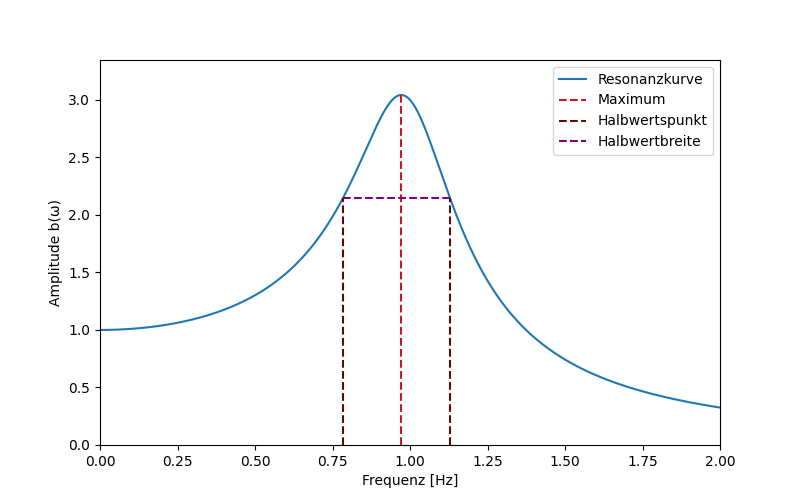
\includegraphics[width=0.5\textwidth]{img/13/Resonanzkurve_allgemein.png}
    \caption{ Schematic resonance curve $b(\omega)$ of a damped, forced oscillator.}
    \label{fig:resonancecurve}
\end{figure}

\textcolor{red}{ADD LABELS FOR THE POINTS IN THE FIGURE HERE!}

Important quantities to characterize the resonance curve are the half-width $H$ and the resonance enhancement:
\begin{equation}
H = \omega_2 - \omega_1 = 2 \delta, \quad \frac{b(\omega')}{b(\omega \to 0)} = \frac{\omega_0}{2 \delta}.
\end{equation}

By measuring free and forced oscillations, the damping constant $\delta$ and the natural frequency of the torsional pendulum can be determined in several ways and compared.

\subsection*{Forces Acting on the System}
The dynamics of the rotary pendulum are determined by the following torques and forces:

\begin{itemize}
    \item \textbf{Restoring torque:} Generated by the torsional stiffness of the pendulum axis, it acts to return the pendulum to its equilibrium position. It is proportional to the angular displacement.
    \item \textbf{Damping torque:} Produced by the eddy current brake. Eddy currents induced in the conductor oppose the motion (Lenz’s law), leading to an angular velocity–dependent resistive torque.
    \item \textbf{Driving torque:} In forced oscillation experiments, the stepper motor provides a periodic torque that excites the pendulum at the frequency set by the function generator.
    \item \textbf{Inertial torque:} Due to the moment of inertia of the pendulum, resisting angular acceleration according to Newton’s second law for rotation.
\end{itemize}

The interplay of these torques determines whether the system undergoes free oscillation, damped oscillation, or driven oscillation.

\subsection*{Influence of Damping on the Resonance Curve}
The resonance curve is characterized by the resonance frequency $\omega'$, the amplitude at resonance $b(\omega')$, and the half-width $H$.

\begin{itemize}
    \item \textbf{Resonance frequency:} With increasing damping, the resonance frequency $\omega'$ shifts to lower values compared to the natural frequency $\omega_0$.
    \item \textbf{Resonance amplitude:} The maximum amplitude $b(\omega')$ decreases as damping increases, since more energy is dissipated per cycle.
    \item \textbf{Half-width:} The half-width $H = 2 \delta$ becomes larger with increasing damping. Thus, the resonance curve broadens as the system becomes less selective in frequency response.
\end{itemize}

In summary, higher damping reduces the resonance peak, shifts it to lower frequency, and widens the curve.

\subsection*{Quality Factor of a Resonator}
The quality factor $Q$ is a dimensionless parameter that characterizes the sharpness of resonance. It is defined as the ratio of the resonance frequency to the half-width of the resonance curve:
\begin{equation}
Q = \frac{\omega_0}{H} = \frac{\omega_0}{2 \delta}.
\end{equation}

A high $Q$ indicates weak damping, a narrow resonance curve, and high resonance amplification. A low $Q$ corresponds to strong damping, a broad resonance curve, and low amplification.
